\documentclass["../Cours.tex"]{subfiles}

\begin{document}
\setcounter{chapitre}{-1}
\chapitre{Opérations sur les nombres relatifs}
\theme{}

\partie{Les nombres}
\souspartie{Les nombres entiers}

\definition{Un nombre \emph{entier naturel} représente une quantité permettant de compter un nombre d'objets.}

\exemple{0 ; 17 ; 43}

\vocabulaire{On parle d'\emph{entier relatif} lorsque l'on parle des entiers positifs et négatifs.}

\remarque{0 est considéré à la fois comme positif et négatif.}

\souspartie{Fractions et nombres rationnels}

\definition{Une fraction est le résultat d'une division entre deux nombres entiers, le numérateur et le dénominateur.}

\exemple{$\dfrac{5}{3}$ est une fraction. $\dfrac{2,4}{7}$ n'est pas une fraction.}

\definition{Un nombre rationnel est un nombre qui peut s'écrire sous forme de fraction.}

\begin{listedexemples}
    \item $\dfrac{7}{2}$ est un nombre rationnel, car c'est une fraction.
    \item $2,5$ est un nombre rationnel, car $2,5 = \dfrac{5}{2}$.
\end{listedexemples}

\clearpage

\souspartie{Les nombres décimaux}

\definition{Une fraction décimale est une fraction dont le dénominateur est égal à 1, 10, 100, \num{1000}, etc.}

\begin{listedexemples}
    \item $\dfrac{84}{100}$ est une fraction décimale, car le dénominateur est 100.
    \item $\dfrac{8}{12}$ n'est pas une fraction décimale, car le dénominateur est 12.
\end{listedexemples}

\definition{Un nombre décimal est un nombre qui peut s'écrire sous forme de fraction décimale.}

\begin{listedexemples}
    \item $7,3$ est un nombre décimal car $7,3 = \dfrac{73}{10}$
    \item $\dfrac{1}{3}$ n'est pas un nombre décimal, en effet $\dfrac{1}{3} = 0,333...$ \\[1em](il y a une infinité de chiffres après la virgule, donc ce n'est pas un nombre décimal)
\end{listedexemples}


\partie{Opérations}
\souspartie{Addition}

\vocabulaire{L'addition décrit la réunion de deux quantités. Elle est notée avec le symbole $+$, les deux nombres additionnés sont les \emph{termes} et le résultat est appelé la \emph{somme}.}

\exemple{$2+3=5$ : les termes sont 2 et 3 ; la somme est 5.}

\propriete{L'addition est \emph{commutative}, c'est-à-dire que l'on obtient le même résultat en intervertissant les deux termes.}

\begin{listedexemples}
    \item $9+8=8+9$
    \item $12+17=17+12$
\end{listedexemples}

\clearpage

\propriete{Pour additionner deux nombres relatifs :
\begin{itemize}
    \item s'ils sont de même signe, la somme a le même signe et on additionne les distances à zéro ;
    \item s'ils sont de signes différents, le signe de la somme est celui du terme de la plus grande distance à zéro, et on soustrait les distances à zéro.
\end{itemize}
}

\souspartie{Soustraction}

\vocabulaire{La soustraction décrit le retranchement d'une quantité à une autre. Elle est notée avec le symbole $-$, les deux nombres sont les termes et le résultat est appelé la \emph{différence}.}

\exemple{$8-5=3$ : les termes sont 8 et 5 ; la différence est 3.}

\propriete{Soustraire un nombre revient à ajouter son opposé.}

\begin{listedexemples}
    \item $(-6) - (-4) = (-6) + (+4)$
    \item $(+8) - (+2) = (+8) + (-2)$
\end{listedexemples}

\souspartie{Multiplication}

\definition{La multiplication est la répétition successive d'une addition. Les nombres multipliés sont les \emph{facteurs} et le résultat est appelé le \emph{produit}.}

\begin{listedexemples}
    \item << 5 fois 2 >> $ = 5 \times 2 = 2+2+2+2+2$
    \item << 3 fois 7 >> $ = 3 \times 7 = 7+7+7$ 
\end{listedexemples}

\propriete{La multiplication est \emph{commutative}, c'est-à-dire que l'on obtient le même résultat en intervertissant les deux facteurs.}

\exemples{$8 \times 7 = 7 \times 8$ ~~~~~~~~~~ $12 \times 4 = 4 \times 12$}

\souspartie{Division}

\vocabulaire{La division permet de séparer en plusieurs parts égales une quantité. On divise le \emph{dividende} par le \emph{diviseur} afin d'obtenir le \emph{quotient} et le \emph{reste}.
Les symboles utilisés pour la division sont les deux-points << : >>, le \textit{slash} << / >> et l'obélus << $\div$ >>.}

\begin{figure}[h!]
    \centering
    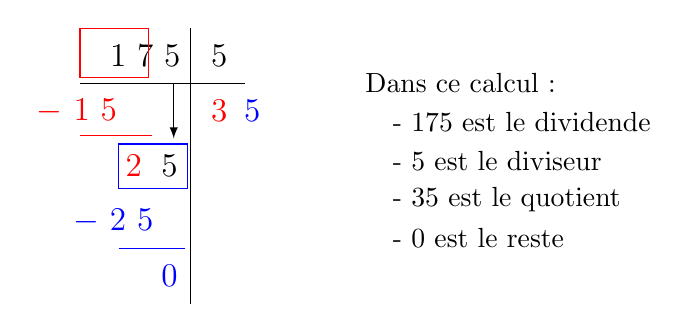
\begin{tikzpicture}[scale=0.7]
        \draw (0,0) -- (3,0);
        \draw (2,1) -- (2,-4);
        \node[anchor=east] at (2,0.5) {\large{$1~7~5$}};
        \node[anchor=west] at (2.2,0.5) {\large{$5$}};
        \draw[red] (0,0.1) rectangle (1.25,1);
        \node[red, anchor=west] at (2.2,-0.5) {\large{$3$}};
        \node[red, anchor=west] at (-0.96,-0.5) {\large{$-~1~5$}};
        \draw[red] (0,-0.95) -- (1.3,-0.95);
        \node[red, anchor=west] at (0.65,-1.5) {\large{$2$}};
        \draw[-latex] (1.7,0) -- (1.7,-1);
        \node[anchor=west] at (1.3,-1.5) {\large{$5$}};

        \draw[blue] (0.7,-1.1) rectangle (1.95,-1.9);
        \node[blue, anchor=west] at (2.8,-0.5) {\large{$5$}};
        \draw[blue] (0.7,-3) -- (1.9,-3);
        \node[blue, anchor=west] at (-0.3,-2.5) {\large{$-~2~5$}};
        \node[blue, anchor=west] at (1.3,-3.5) {\large{$0$}};

        \node[anchor=west] at (5,0) {Dans ce calcul :};
        \node[anchor=west] at (5.5,-0.7) {- $175$ est le dividende};
        \node[anchor=west] at (5.5,-1.4) {- $5$ est le diviseur};
        \node[anchor=west] at (5.5,-2.1) {- $35$ est le quotient};
        \node[anchor=west] at (5.5,-2.8) {- $0$ est le reste};
    \end{tikzpicture}
    \caption{Exemple de division posée}
\end{figure}


\clearpage
\partie{Priorité opératoire}

\propriete{Dans un calcul contenant plusieurs opérations :
    \begin{itemize}
        \item la priorité est donnée aux calculs entre parenthèses,
        \item puis, aux multiplications et aux divisions (de gauche à droite),
        \item enfin, aux additions et aux soustractions (de gauche à droite).
    \end{itemize}
}

\exemple{$$A = (7 + \underline{15 \div 3}) \times 3$$  $$A = \underline{(7+5)} \times 3$$ $$A = \underline{12 \times 3}$$ $$A = 36$$}

\remarque{Dans un calcul contenant un trait de fractions, on calcule d'abord le numérateur et le dénominateur, puis on effectue la division.}

\exemple{$$\dfrac{17+3}{15-5} = \left(17+3\right) \div \left(15-5\right)$$}


\end{document}